\documentclass[11pt,a4paper]{article}
\usepackage[utf8]{inputenc}
\usepackage{amsmath}
\usepackage{amsthm}
\usepackage{amsfonts}
\usepackage{amssymb}
%\usepackage{algorithmic}
%\usepackage{algorithm}
\usepackage{hyperref}
%\usepackage[ruled,linesnumbered,procnumbered]{algorithm2e}

\makeatletter
\let\original@algocf@latexcaption\algocf@latexcaption
\long\def\algocf@latexcaption#1[#2]{%
  \@ifundefined{NR@gettitle}{%
    \def\@currentlabelname{#2}%
  }{%
    \NR@gettitle{#2}%
  }%
  \original@algocf@latexcaption{#1}[{#2}]%
}
\makeatother

\usepackage{xcolor}		% for adding colors to the text

\usepackage[footnotesize, center]{caption}	
\usepackage{subcaption}
%\usepackage{subfigure}
\usepackage{booktabs}
\usepackage{multirow}
\usepackage{breakurl}	% fixes the problem of breaking long url into lines inside the bibliography (IMP: must be below the hyperref package)
\hypersetup{
    bookmarks=true,		% show bookmarks bar?
    colorlinks=true,		% false: boxed links; true: colored links
    linkcolor=blue,		% color of internal links
    citecolor=blue,		% color of links to bibliography
    filecolor=blue,		% color of file links
    urlcolor=blue,		% color of external links
    bookmarksopen=true,
    breaklinks=true,
}
%\usepackage{natbib}			% bibliography
%\setlength{\bibsep}{0pt}

\usepackage[title]{appendix}

\usepackage{longtable}

% Page Setup

% Margins
	% MS Word (Default):		[margin=0.98in]
	% MS Word (Narrow):		[margin=0.5in]
\usepackage[margin=2cm]{geometry}
\setlength{\parskip}{\medskipamount}

\usepackage{setspace}
%\onehalfspacing
\setstretch{1.15}

\usepackage{indentfirst}			% indent the first paragraph
\allowdisplaybreaks				% break if equations take too much vertical space

% Section Style
\makeatletter
\def\@seccntformat#1{\csname the#1\endcsname.\quad}		% put a fullstop after section numbers
\makeatother

% Optional packages
\usepackage{xfrac}	% nicer fractional symbols (e.g., \sfrac{1}{2})
\usepackage{fancyhdr}	% adding headers / footers

% MACROS

% mathematical
\newcommand{\mathbold}[1]{\boldsymbol{#1}}		% for adding bold greek letters
\newcommand{\binary}{\{ 0, 1 \} }

\newcommand{\parentheses}[1]{\left( #1 \right) }	% auto-size parentheses
\newcommand{\brackets}[1]{\left[ #1 \right] }		% auto-size brackets
\newcommand{\curly}[1]{\left\{ #1 \right\} }		% auto-size curly brackets

	% Nilay Noyan's commenting macros
	% commentbox (adds black comments in a frame box)
	% comment (adds red comments as a footnote)

\newcounter{commentcounter}
\setcounter{commentcounter}{1}

\setlength{\fboxsep}{5pt}
\setlength{\fboxrule}{0.1pt}

\newcommand{\commentbox}[1]{
% \hfill \newline \noindent
%	\framebox[\textwidth]{
%		\parbox{0.98\textwidth}{
%			\footnotesize{
%				\texttt{\textcolor{black}{(C.\arabic{commentcounter})~#1\hfill}}}}}
%	\addtocounter{commentcounter}{1} 
	}

\long\def\symbolfootnote[#1]#2{\begingroup\def\thefootnote{\fnsymbol{footnote}}\footnote[#1]{#2}\endgroup}

\newcommand{\comment}[2]{{\footnotesize\texttt{\textcolor{red}{(C.\arabic{commentcounter})}}\symbolfootnote[4]{\texttt{\textcolor{red}
        {(C.\arabic{commentcounter}) [#1]: ~#2}}}}\addtocounter{commentcounter}{1}}
%\newcommand{\comment}[2]{}

% theorems
% the subtheorem environment is used to generate theorem numbers 1a, 1b, etc.
% Source: http://tex.stackexchange.com/questions/43346/how-do-i-get-sub-numbering-for-theorems-theorem-1-a-theorem-1-b-theorem-2
\makeatletter
\newenvironment{subtheorem}[1]{%
  \def\subtheoremcounter{#1}%
  \refstepcounter{#1}%
  \protected@edef\theparentnumber{\csname the#1\endcsname}%
  \setcounter{parentnumber}{\value{#1}}%
  \setcounter{#1}{0}%
  \expandafter\def\csname the#1\endcsname{\theparentnumber\alph{#1}}%
  \ignorespaces
}{%
  \setcounter{\subtheoremcounter}{\value{parentnumber}}%
  \ignorespacesafterend
}
\makeatother
\newcounter{parentnumber}
% end of subtheorem environment

\newtheorem{theorem}{\bf Theorem}
\newtheorem{lemma}{\bf Lemma}
\newtheorem{proposition}{\bf Proposition}
\newtheorem{corollary}{\bf Corollary}
\newtheorem{definition}{\sc Definition}
\newtheorem{fact}{\bf Fact}
\newtheorem{claim}{\sc Claim}
\newtheorem{case}{\sc Case}
\newtheorem{observation}{\sc Observation}
\renewcommand{\qedsymbol}{\hfill \tiny$\blacksquare$}		% symbol for proof environment
\renewcommand{\proofname}{\textnormal{\textbf{Proof.}}}	% title in the proof environment

\newtheoremstyle{mytheoremstyle} % name
    {\topsep}                    % Space above
    {\topsep}                    % Space below
    {}                   % Body font
    {}                           % Indent amount
    {\scshape}                   % Theorem head font
    {.}                          % Punctuation after theorem head
    {.5em}                       % Space after theorem head
    {}  % Theorem head spec (can be left empty, meaning ‘normal’)
\theoremstyle{mytheoremstyle}
\newtheorem{example}{Example}

\newtheoremstyle{myassumptionstyle} % name
    {\smallskipamount}                    % Space above
    {0}                    % Space below
    {}                   % Body font
    {}                     	% Indent amount
    {\upshape}              % Theorem head font
    {.}                          	% Punctuation after theorem head
    {.5em}                      % Space after theorem head
    {}  				% Theorem head spec (can be left empty, meaning ‘normal’)
\theoremstyle{myassumptionstyle}
\newtheorem{assumption}{\bf A\ignorespaces}
\newtheorem{remark}{\bf Remark}

\DeclareMathOperator*{\argmin}{arg\,min} 
\DeclareMathOperator*{\argmax}{arg\,max} 


% narrative
\newcommand{\ie}{\textit{i.e.}}		% id est, that is to say
\newcommand{\ex}{\textit{ex.}}		% example
\newcommand{\eg}{\textit{e.g.}}	% exempli gratia, for the sake of example

\newcommand{\st}{\text{subject to:}\qquad}	% subject to
\newcommand{\mathbi}[1]{\boldsymbol{#1}}	% \boldsymbol{ any character } // makes both italic and bold

\newcommand{\cplex}{\texttt{CPLEX}}

\newcommand{\question}[1]{\vspace{\baselineskip}\noindent\pdfbookmark{Question #1}{Question #1}\textbf{\large{Question #1}} \normalsize\medskip\newline}
\newcommand{\qpart}[1]{\indent\textbf{#1)}}	% i.e., a), b), ...

\newcommand{\inlinecomment}[1]{{\color[rgb]{0.13,0.57,0.4} \textbf{#1}}}

% algorithmic
\newcommand{\np}{$\mathcal{NP}$}	% e.g., as in NP-hard

\usepackage{enumitem}	% for aligned descriptions
\usepackage{calc} 		% for aligned descriptions

\setenumerate{
itemsep=0pt,
partopsep=0pt,
parsep=0pt,
topsep=0pt,
labelindent=4pt,
font=\normalfont
}

\setdescription{
itemsep=0pt,
partopsep=0pt,
parsep=0pt,
topsep=0pt,
labelindent=4pt,
font=\normalfont
}

\setitemize{
itemsep=0pt,
partopsep=0pt,
parsep=0pt,
topsep=0pt,
labelindent=4pt,
font=\normalfont
}


\setlength{\textheight}{23cm} %{23cm}
\setlength{\topmargin}{-2cm}
\setlength{\textwidth}{17.5cm} \setlength{\oddsidemargin}{-0.5cm}
\setlength{\evensidemargin}{-0.5cm}

\setlength{\parindent}{0pt}

\newcommand{\gap}{\vspace{5pt}}
\newcommand{\epc}{\hspace{1pc}}

\newcommand{\onebld}{{\bf 1}}
\newcommand{\wt}{\widetilde}
\newcommand{\wh}{\widehat}

\newcommand{\E}{{\rm I\!E}}
\newcommand{\IP}{{\rm I\!P}}
\newcommand{\D}{{\rm I\!D}}
\newcommand{\pmat}[1]{\begin{pmatrix} #1 \end{pmatrix}}
\newcommand{\us}[1]{{\color{black}#1}}
\newcommand{\ssbs}[1]{{\color{blue}#1}}
\bibliographystyle{plain}

%% Semih's additions %%
\usepackage{mathtools}
%% end of semih's additions %%


\title{\bf Taming the Duck: Can Stochastic Programming Help?}
\date{}
%\author{Harsha Gangammanavar\\Engineering Management, Information, and Systems\\Southern Methodist University, \\ Dallas, TX 75275}

\begin{document}
\pagenumbering{gobble}
\maketitle

\vspace*{-1.3cm}

\paragraph{Suvrajeet Theodore Sen:} 
The Quandary of Renewable Energy Integration

Lawmakers throughout the U.S. have mandated that electricity supply should include a significant percentage of energy from renewable resources - each state has set its own goal, with California being most aggressive requiring 50\% renewable energy by 2030.  Local/State authorities (e.g., Independent System Operators (ISO)) which are in-charge of wholesale electricity supply have commissioned focused studies to assess operational considerations such as system reliability, market design, storage technologies and other devices.  However a recent study commissioned by CAISO (see Olson et al 2015) suggest that for penetration levels beyond 33\%, there one can expect a great deal of over-generation  while also facing the possibility of curtailment of renewable energy, or load-shedding in the evening.  In case of curtailment of renewable energy, one faces the likelihood of negative prices in the market leading to large shipments of energy to neighboring states (e.g., Arizona) while paying those states to accept electricity from California. For the case of load-shedding, the loss of load probability (or loss of load expectation) can reach unacceptable levels, affecting system performance.  Page restrictions limit us from getting into more detailed discussions on the impact on GHG emissions due to the use of so-called fast-generators.  As these complications play out within the ISO communities, researchers in some environmental science programs have published a well-cited study in the Proceedings of the National Academy of Science (PNAS) where the authors suggest that renewable energy can be used to power 100\% of electricity requirements by 2050  (Jacobson et al 2017).  This study has come under heavy fire from a large group of engineers (Clack et al 2017) because the PNAS paper did not accommodate many engineering considerations such as transmission capacity, reliability and the like.   In addition to these considerations, the Federal Energy Regulatory Commission (FERC) has mandated that due to the volatility of renewable generators (solar and wind), electricity dispatch must take place at 10-15 minute intervals, instead of the usual hourly interval, which is the norm for fossil-fuel generators.  Such shorter dispatching intervals can help the system track changes in renewable generation.  However, these shorter time scales also calls for faster algorithms and faster computing environments.  In any event, it is important to recognize that just like any other infrastructure, reliability and efficient system operation requires us to strike a delicate balance between multiple facets such as generators, grids, natural resources, the weather, and of course market economics and public policy.  
The following is a small test grid example which is intended for academic tests of power system models. It is referred to as IEEE 118 (with 118 nodes/buses). Using the above network as a sample for experimenting with renewable energy, the National Renewable Energy Lab (NREL) has created a similar instance (called NREL 118) which represents a small grid (with 118 buses) and includes renewable resources together with conventional generators, and a transmission grid.  In addition, one can include market forces, weather models, and alternative renewable penetration policies to setup semi-realistic models which include statistical representations of wind, solar, and weather, economic representation of market equilibria, and operational models of resource utilization, reliability constraints and the like.  Such models have become an integral part of the OE community.  Our goal is to make realistic experimentation possible by allowing new models and algorithms for some aspects of the system, while leveraging the remaining data, models, and algorithms of a cyberinfrastructure which would be supplied within CORE.   A typical researcher who may  have an interest and expertise creating a new sub-model and/or algorithm, would be able to experiment with their new model/algorithm  by replacing the some of the functions of the CORE setup with their own trial  model/algorithm, while leveraging the remainder of the model/algorithm included within CORE.  In this way, the research community will be able to carry out experiments which test the approach within the broader context of the application.  Such experimentation will have the ability to establish benchmarks which are much more realistic than is available today. 
[1]	Clack, C.T.M. et al, 2017, “Evaluation of a proposal for reliable low cost grid power with wind, water, solar” Proceedings of the National Academy of Sciences, 114(26): 6722-6727.
[2]	Jacobson M. Z, et al. 2015, “100\% clean and renewable wind, water, and sunlightc(WWS) all-sector energy roadmaps for the 50 United States,”  Energy Environ Sci. 8:2093–2117.
[3]	Olson, A. et al 2015, “Halfway There:  Can California Achieve a 50\% Renewable Grid,” IEEE Power and Energy Magazine, 13(4): 41-93.


\paragraph{Harsha:} Renewable energy resources constitute a significant fraction of the nation's energy portfolio. It is expected that their contribution will increase at an astonishing $5\%$/year for the next $25$ years \cite{AEO2016}. A large portion of the forecasted renewable capacity addition will be provided by solar (from $25$ GW in 2015 to $246$ GW in 2040), followed by wind installations ($73$ GW between 2015 and 2040). While wind generation is hampered by the need to install new transmission lines to access remote wind sites, investments in solar generation has surged in recent years and it is expected to surpass wind capacity by 2032 \cite{AEO2016}. In any case, both these renewable resources exhibit three key characteristics: (a) variability - high magnitude changes in output in short duration of time, (b) uncertainty - unpredictable output, and (c) non-dispatchability - output limited to certain time periods in a day which does not coincide with demand. 

\gap{}

Variability and uncertainty of solar and wind generation pose significant technological and operational challenges, especially at high penetration levels. A particular difficulty arises due to frequent and large energy imbalances between total available resources and demand. These imbalances are addressed by system operators through procurement of additional operating reserves for short time frames (usually $5-60$ minutes). In our previous work \cite{Gang16a}, we have established that the amount of operating reserves necessary to maintain system reliability will increase with penetration of renewable resources. Serving half (as is the case in California \cite{SB350}) of the electric load with wind and solar requires an unprecedented level of these reserves. 

\gap

\begin{figure}
\centering
\vspace*{-0.6cm}
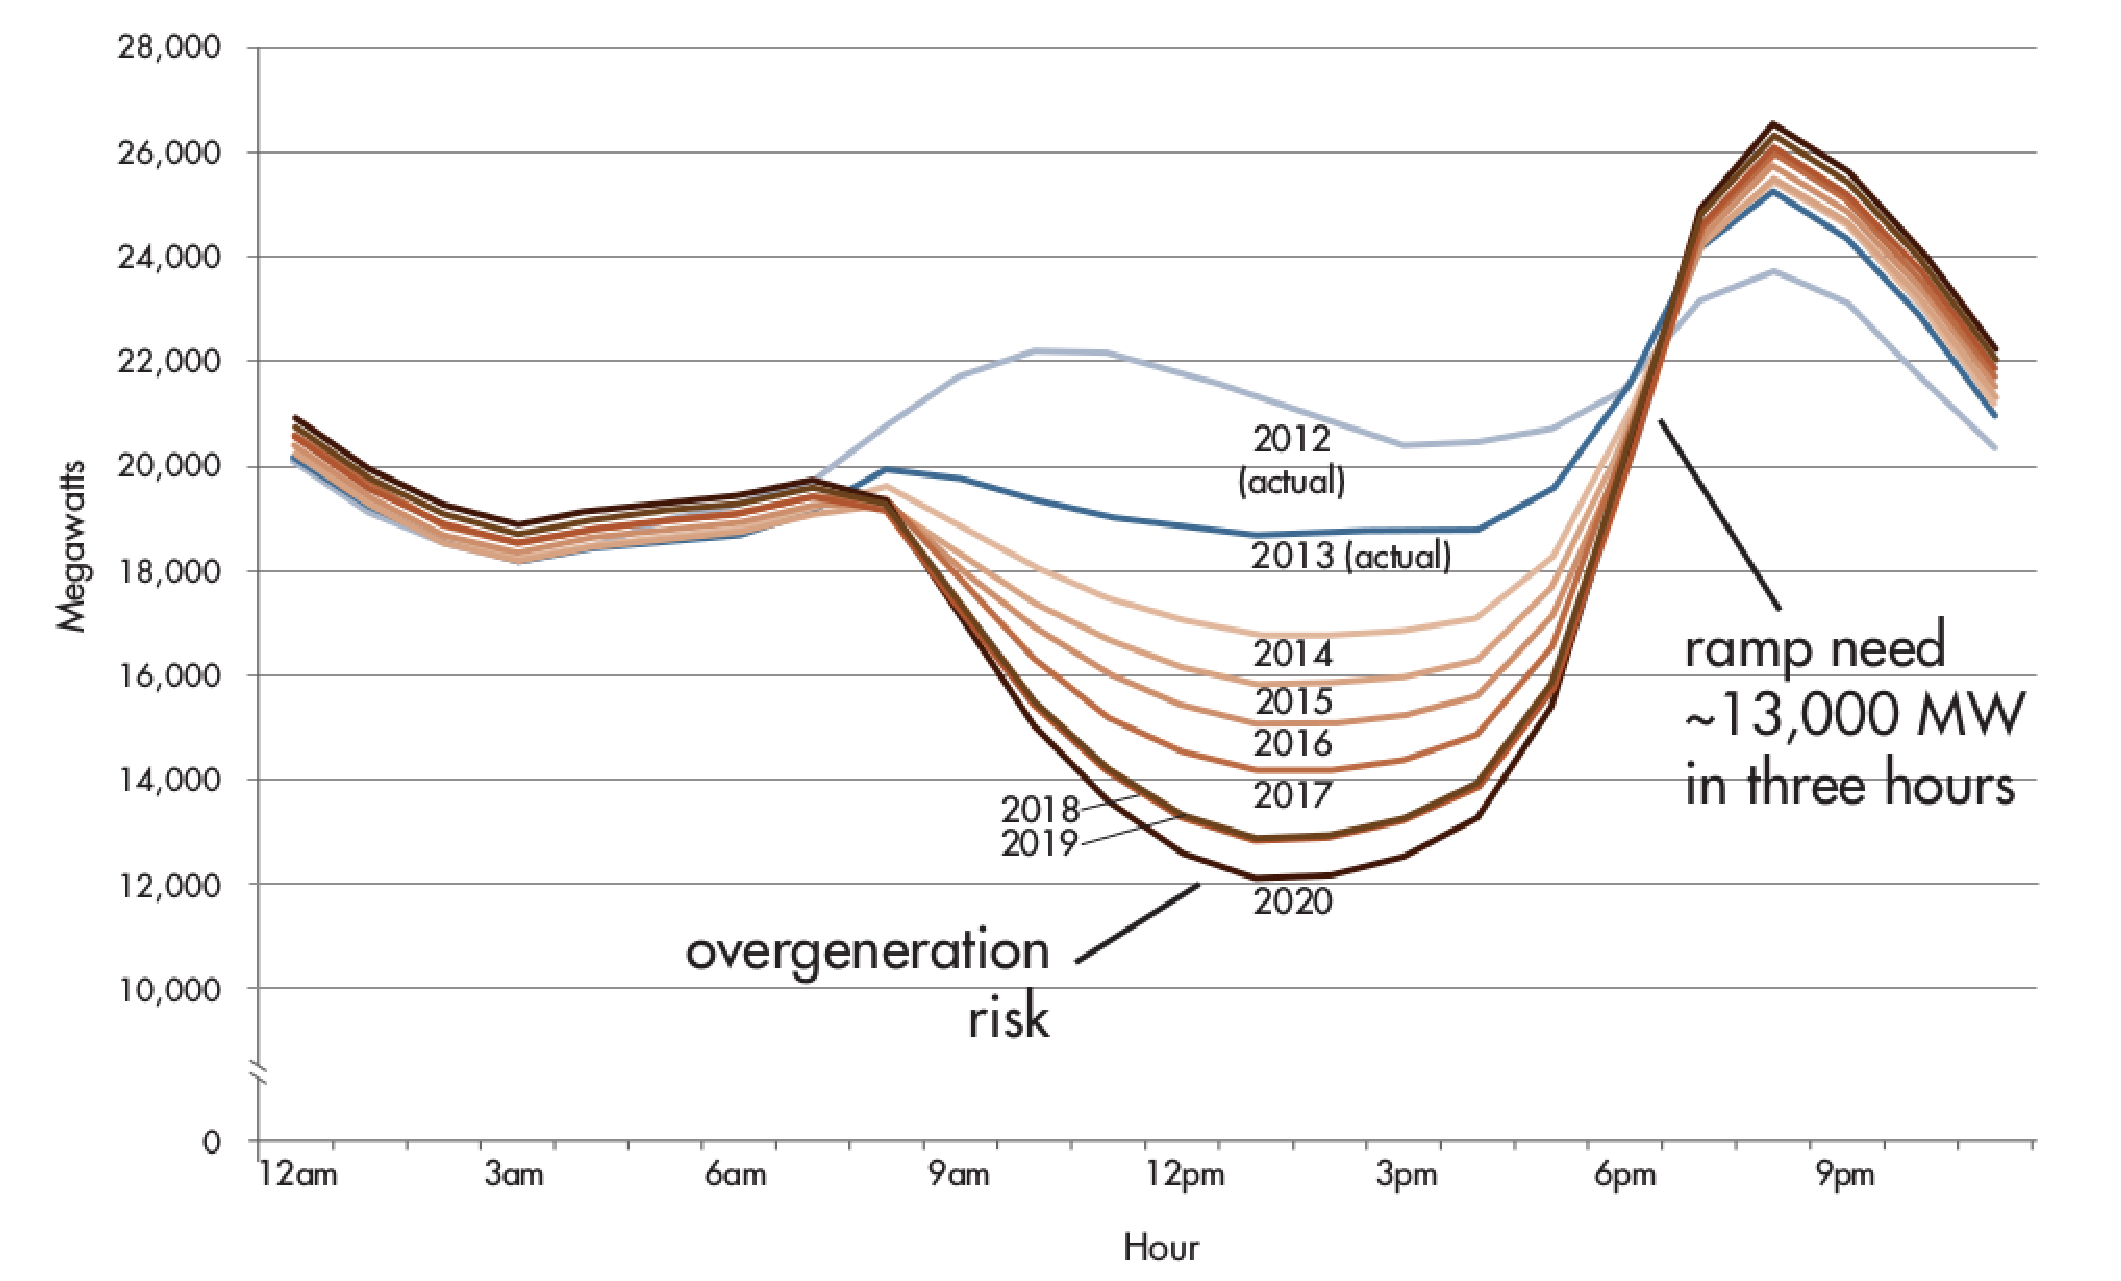
\includegraphics[scale=0.2]{./figures/duckChart}
\caption{CAISO's duck chart} \label{fig:duck}
\end{figure}

Non-dispatchability of wind and solar poses an even larger challenge for power system design. This is best illustrated in the widely circulated ``duck chart'' by California Independent System Operator (CAISO) which shows the net-load (difference between demand and generation) profile over successive years as more solar is installed \cite{Duck16}. The figure illustrates that the combination of increased load in the evening and reduction of solar generation at sundown creates a significant requirement for upward ramp. This may result in (1) an inability to meet the evening hour load due to insufficient upward ramping capability resulting in the undesirable load curtailment, (2) curtailment of renewable resources in the afternoon and allowing additional conventional generation to stay online, which reduces the effective capacity value of renewable resources and increases risk of over generation, and (3) procure sufficient upward ramping capability. The latter option has prompted CAISO and California Public Utilities Commission to propose ``flexible resource adequacy criteria and must offer obligations'' which requires California utilities to procure sufficient upward ramping capability \cite{FracMoo16}. These fast ramping reserves use fossil fuels (mainly, natural gas) and therefore undermine the original drive towards renewable resources, namely, reduction in CO2 emissions.

\gap

In light of these observations, our main questions are the following: (a) \textit{Is the power system reserve sufficient to support an ever-increasing renewable portfolio standards?}. We term a power system to be ``reserve sufficient'' if it has adequate reserves to maintain reliable operations at a certain renewable penetration level without undermining emission targets. (b) \textit{What is the impact of using advanced stochastic optimization tools for scheduling generators and operating reserves in power systems? Will it help achieve reserve sufficiency?} To achieve this we need:
\begin{enumerate} \itemsep0em
	\item {\it Develop reserve sufficiency models} which include different types of operating reserves, physical constraints of the power network, uncertainty in generation and demand, and differences in operating timescales of generators in the system. These models should capture the trade-off between an increase in renewable penetration and an increase in CO2 emissions from higher operating reserve utilization.
	\item {\it Develop an integrated stochastic optimization framework} which combines optimization and simulation. These stochastic frameworks should capture all the three characteristics of renewable generation and hence, offer an effective tool to establish reserve sufficiency.
\end{enumerate}

{\bf Design and Methodology}: Our framework uses suite of multiperiod stochastic programs that can be decomposed into a computationally viable form. Our preliminary model instances will be based on standard IEEE test systems \cite{Chri99}, which will then be scaled to a more realistic instance based on the Illinois power system used in \cite{Gang16a}. The uncertainty quantification related to renewable generation and demand will be based on open-access databases, such as WWSIS \cite{Pott08}. Our stochastic framework will use the stochastic mixed-integer Benders decomposition for commitment problems and two-stage stochastic decomposition \cite{Higl94} for economic dispatch as the optimization engines, and novel techniques to capture the hierarchical dynamics across time periods of operation. The focus will be on developing models that can be solved in a parallel/distributed environment high-performance computing resources. 

\paragraph{Semih:} 

\section{Hierarchical Decision Process}
We consider a hierarchy of decision processes which involves three components (a) long-term unit-commitment, (b) short-term unit-commitment, and (c) economic dispatch. 

\subsection{Unit-commitment Formulation}
We consider a set of generators $\mathcal{G}$ that needs to be scheduled within a planning horizon, defined by a set of time periods $\mathcal{T}$. In a feasible schedule, all generators must obey their physical capabilities. We begin with introducing the parameters ($\forall i \in \mathcal{G}$) to model generator limitations.
\begin{description} \setlength{\itemsep}{-1pt}
\item{$G_i^{\max}$:} Maximum generation capacity, 
\item{$G_i^{\min}$: } Minimum required production amount when the generator is online, 
\item{$\Delta G_i^{\max}$: } Ramp up limit, 
\item{$\Delta G_i^{\min}$:} Ramp down limit,
\item{$UT_i$:} Minimum required uptime before the generator can become offline, 
\item{$DT_i$:} Minimum required downtime before the generator can become online,  
\end{description}

In order to model the commitment decisions, we first define the state of a generator at a particular time period. Our definition is based on the online/offline status of the generator. In particular, we consider a generator as online whenever its output is at least $G_{i}^{\min}$, and label it as offline if otherwise. Note that this definition allows a generator to be operational even though it is offline (e.g., when the generator is ramping up towards $G_{i}^{\min}$ after it has been turned on). Accordingly, we define the following binary variables:

\begin{description} \setlength{\itemsep}{-1pt}
\item{$x_{it}$:} 1 if generator $i$ is operational at $t$, 0 otherwise,
\item{$s_{it}$:} 1 if generator $i$ becomes online at $t$, 0 otherwise,
\item{$z_{it}$:} 1 if generator $i$ becomes offline at $t$, 0 otherwise.
\end{description}

The generation amounts ($\forall i \in \mathcal{G}$) will be determined by the following decision variables:

\begin{description}\setlength{\itemsep}{-1pt}
\item{$G_{it}$:} Output of generator $i$ at time $t$,
\end{description}

The formulation is stated below.
\begin{subequations}
\begin{align}
\begin{split}
\min \quad \sum_{i \in \mathcal{G}} \sum_{ t \in \mathcal{T} } c^{gen}_{i} G_{it} + c^{start}_i s_{it} + c^{noload}_i x_{it} 
\end{split}
\\ 
\text{s.t.} \qquad \quad & \parbox{2cm}{\it \small State \newline Equations} 
\begin{dcases}
x_{it} - x_{it-1}  = s_{it} - z_{it},  & \forall i \in \mathcal{G}, \, t \in \mathcal{T}, \label{con:state_transition} \\ 
x_{it}, \, s_{it}, \, z_{it} \in \{ 0 , 1 \}, & \forall i \in \mathcal{G}, \, t \in \mathcal{T}.
\end{dcases}  \\ 
%
& \parbox{2cm}{\it \small Generation \newline Limits}
\begin{dcases}
G_i^{\min} x_{it} \leq G_{it} \leq G_i^{\max} x_{it}, & \forall i \in \mathcal{G}, \, t \in \mathcal{T}, \label{con:gen_limits} 
\end{dcases} \\
% 
& \parbox{2cm}{\it \small Ramping \newline Restrictions} 
\begin{dcases} 
 \Delta G_i^{\min} \leq G_{it} - G_{it-1} \leq \Delta G_i^{\max}, & \forall i \in \mathcal{G}, \, t \in \mathcal{T}, \label{con:ramping} 
\\ 
\end{dcases} \\
%
& \parbox{2cm}{\it \small Minimum Up/Down Restrictions}
\begin{dcases}
 \sum_{j=t-UT_i+1}^{t-1} s_{ij} \leq v_{it}, & \forall i \in \mathcal{G},\, t \in \mathcal{T}, 
%\label{con:min_uptime} 
\\ 
 \sum_{j=t-DT_i}^{t} s_{ij} \leq 1-v_{it}, & \forall i \in \mathcal{G}, \, t \in \mathcal{T}, 
%\label{con:min_downtime}
\label{con:min_updown}
\end{dcases}
\end{align}
\end{subequations}
In the above formulation, the commitment decisions are determined in  \eqref{con:state_transition}, the generation limits are modeled in \eqref{con:gen_limits}. Ramping and minimum uptime/downtime restrictions are modeled using \eqref{con:ramp_updown} and \eqref{con:min_updown}, respectively. Constraints \eqref{con:variable_cost} determines the amounts of generation at each cost level, which is eventually used to determine a piecewise-linear generation cost approximation in the objective function. Similarly, constraints \eqref{con:startup_cost} models the piecewise-linear approximations of the nonlinear start up costs. Note that the first piece of the start up cost is accounted in the objective with $s_{it}$ variables, therefore the constraints \eqref{con:startup_cost} will only determine the remaining portion of the cost. In this study, we assume that the nuclear and hydroelectric generators are always online, \ie, $s_{it} + v_{it} = 1$. 




\newpage
{\bf Backdrop}: 
\begin{enumerate}
\item {\it ``Scheduling and Pricing for Expected Ramp Capability in Real-Time Power Markets''}: Variability is easier to accommodate than uncertainty. Since the changes are known, it can be scheduled for as long as the flexibility is available and resources are willing to provide it. It is possible that the capabilities of the supply mix are insufficient, and that even if the ramp required is known, the aggregate response speed is not capable of meeting it. When there is sufficient flexibility, the majority of expected variability that occurs on the system can usually be met explicitly through the previously discussed scheduling models. There are a few exceptions. First, it is possible that the variability is occurring at faster resolution than the scheduling model, and not enough information is available to meet this variability explicitly. Second, it is possible that the expected variability occurring in the future can affect the decisions that must be made now, and that information
is beyond the scheduling horizon and not used within the scheduling model. 
\end{enumerate}

\newpage
\begin{thebibliography}{9}

\bibitem{AEO2016}
    \emph{``Annual Energy Outlook''}, 2016, U.S. Energy Information Administration, DOE/EIA-0383.

\bibitem{Gang16a}
	H. Gangammanavar, S. Sen and V. M. Zavala, \emph{``Stochastic Optimization of Sub-Hourly Economic Dispatch With Wind Energy,''} in IEEE Transactions on Power Systems, vol. 31, no. 2, pp. 949-959, March 2016.

\bibitem{Gang16b} H. Gangammanavar and S. Sen, \emph{``Two-scale Stochastic Optimization for Controlling
Distributed Storage Devices,''} accepted for publication in IEEE Transactions on Smart Grid, 2016.

\bibitem{SB350}  California Legislative Information, \emph{``SB-350 Clean Energy and Pollution Reduction Act of 2015''} , Sacramento, CA, October 7, 2015.

\bibitem{Duck16} \emph{``California ISO - Fast Facts''} available at \href{https://www.caiso.com/Documents/FlexibleResourcesHelpRenewables_FastFacts.pdf}{https://www.caiso.com}.

\bibitem{FracMoo16} \emph{``Flexible resource adequacy criteria and must offer obligations''}, available at \href{https://www.caiso.com/informed/Pages/StakeholderProcesses/FlexibleResourceAdequacyCriteria-MustOfferObligations.aspx} {https://www.caiso.com}.
%\bibitem{FracMoo16} \emph{``​Flexible resource adequacy criteria and must offer obligations''}, available at \href{https://www.caiso.com/informed/Pages/StakeholderProcesses/FlexibleResourceAdequacyCriteria-MustOfferObligations.aspx} {https://www.caiso.com}.

\bibitem{Chri99} R. D. Christie, \emph{``Power Systems Test Case Archive''}, available at \href{http://www.ee.washington.edu/research/pstca/} {http://www.ee.washington.edu/research/pstca/}, 1999.

\bibitem{Pott08} C. W. Potter, et al., \emph{``Creating the Dataset for the Western Wind and Solar Integration Study ({U}.{S}.{A}.)''}, Wind Engineering, vol. 32, no. 4, pp. 325-338, 2008.

\bibitem{Higl94} J.L. Higle, and S. Sen, \emph{``Finite master programs in regularized stochastic decomposition''}, Mathematical Programming, vol. 67, pp. 143-168, 1994.

\bibitem{Olso15} A. Olson et al., \emph{``Halfway There: Can California Achieve a 50\% Renewable Grid?},'' in IEEE Power and Energy Magazine, vol. 13, no. 4, pp. 41-52, July-Aug. 2015.

\end{thebibliography}

\newpage

\end{document}
